The \notreVocabulaire{agent sensors} is the principal piece in the network. Its role is to analyse the data given by a sensor (in this case a camera) and to cooperate with the other \notreVocabulaire{agents sensors} to compare similarities in data gathered. This cooperation aims mainly to reduce noise and avoid obstructions. It also helps to take a decision to set senors in a suitable configuration, if they can move.\\

The starting point of the agent nature is the first criteria stated at the top of section \ref{Agent_newtork_conceptualization}, the goal is to reduced the communication not to overload the system when to many agents are used.First of all the agent create a virtual situation based on information collected in the real situation. The information is either obtained thanks to a sensor or by communication means. Each agent has thereby its own belief of the real situation and uses it to take decision. The second point is that each algorithm is linear, then when two agents have the same beliefs they will act in the same way.\\

\begin{wrapfigure}{r}{10cm}
    \centering
    \includegraphics[page=2,clip,width = 10cm]{systeme_multi_agent/conceptualization/multi_agent_schematic.pdf}
    \caption{Description of belief}
    \label{fig:Belief_description}
\end{wrapfigure}

Assuming now that agents have always the same believes  then they can coordinate themselves without communicating. They are able to predict how they would act if they were in the situation of the other agents thus communication is no more required. This  hypothesis is to strong, in practice believes diverges and communication is partially use to synchronise them.\\


The figure \ref{fig:Belief_description} illustrate how the above principle works. The belief is the one from agent 3. Part of the information comes from the sensors and the rest is sent by the other agents. In this case agent 5 will send an information about target 5 to agent 3. This information is added between the old and the new belief. One can also notice that agent 4 is not represented in the belief. This represent a situation where agent 4 is inactive and thus agent 3 cannot anticipate what it is doing. This small example already shows how hard it is to keep all the believes synchronised.\\

Based on this beliefs the agent is the able to act. This behaviour is described in the section \ref{agent_camera_implementation} because it is specific to the given use case described in section \ref{Use_case}.




